\documentclass[a4]{scrartcl}

% \usepackage[ngerman]{babel}
\usepackage[utf8]{inputenc}
\usepackage{mathtools}
\usepackage{amsmath}
\usepackage{amssymb}
\usepackage{geometry}
\usepackage{scrlayer-scrpage}
\usepackage{float}
\usepackage{xcolor}
\pagestyle{scrheadings}
\clearscrheadfoot

\usepackage[backend=biber, maxbibnames=99]{biblatex}
\addbibresource{references.bib}

\setlength{\parindent}{0cm}


\geometry{
  paper=a4paper, % Change to letterpaper for US letter
  top=2cm, % Top margin
  bottom=1.5cm, % Bottom margin
  left=2cm, % Left margin
  right=3cm, % Right margin
}

\ohead{\\
Pina Kolling\\
piko0011}

\usepackage[framemethod=TikZ]{mdframed}

% Style %
\mdfdefinestyle{enviStyle}{
   innertopmargin = 10pt,
  linewidth      = 1pt,
  frametitlerule = true,
  roundcorner    = 2pt%
}


\newenvironment{CountingDefinition}[2][]{%
   \ifstrempty{#1}%
   {\mdfsetup{%
      frametitle={{\strut ~}}}
   }%
   {\mdfsetup{%
      frametitle={{\strut ~#1}}}%
   }%
   \mdfsetup{
      nobreak                   = true,
     linecolor                 = gray,
    frametitlebackgroundcolor = gray!50,
    style                     = enviStyle
   }
   \begin{mdframed}[]\relax%
   \label{#2}}{\end{mdframed}}

\begin{document}
















%--------------------------------------------------------------------------------------------------------------




\section*{Summary: Lecture 10}

Summary for the chapters \textit{11.1} up to page 245 and \textit{11.2} (page 258 optional). \cite{book, CC}

\begin{CountingDefinition}[Randomized algorithms]{def:validLabelPlacement}
Algorithms based on randomization.


(The algorithm employs a degree of randomness as part of its logic or procedure.)
\end{CountingDefinition}

















%--------------------------------------------------------------------------------------------------------------



\subsection*{Bipartite matching}

\begin{CountingDefinition}[Bipartite Graph]{def:validLabelPlacement}
A graph $G = (U,V,E)$ is called bipartite if the vertices can be divided into two disjoint and independent sets $U$ and $V$. (There are no edges between two elements of $U$ or two elements of $V$).

\begin{figure}[H]
\begin{center}
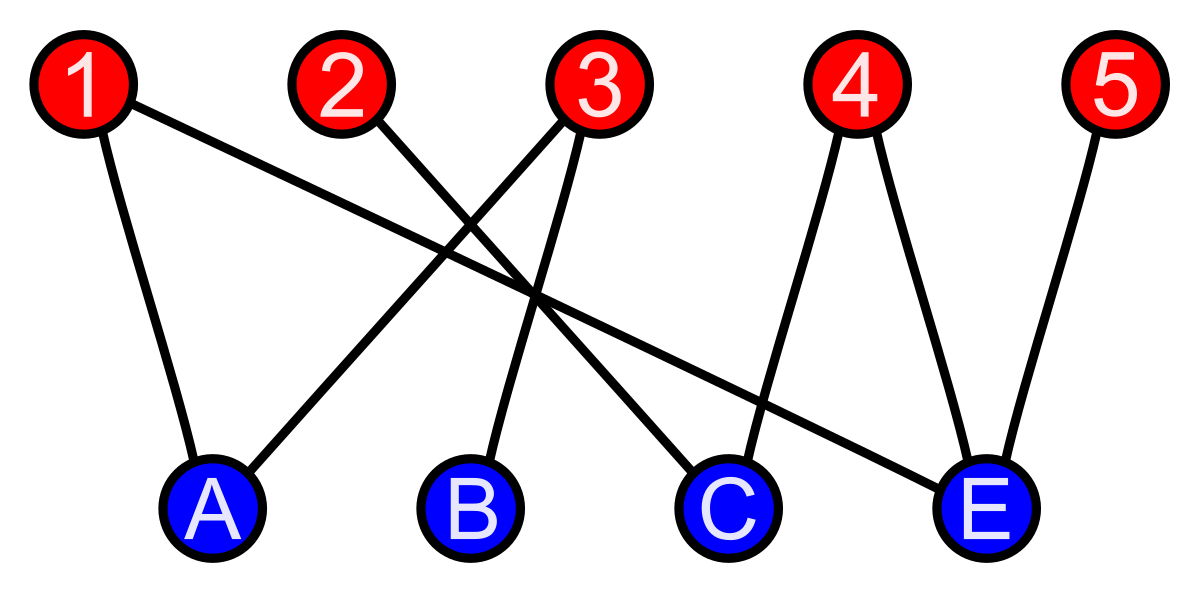
\includegraphics[scale=0.12]{bg1.png}
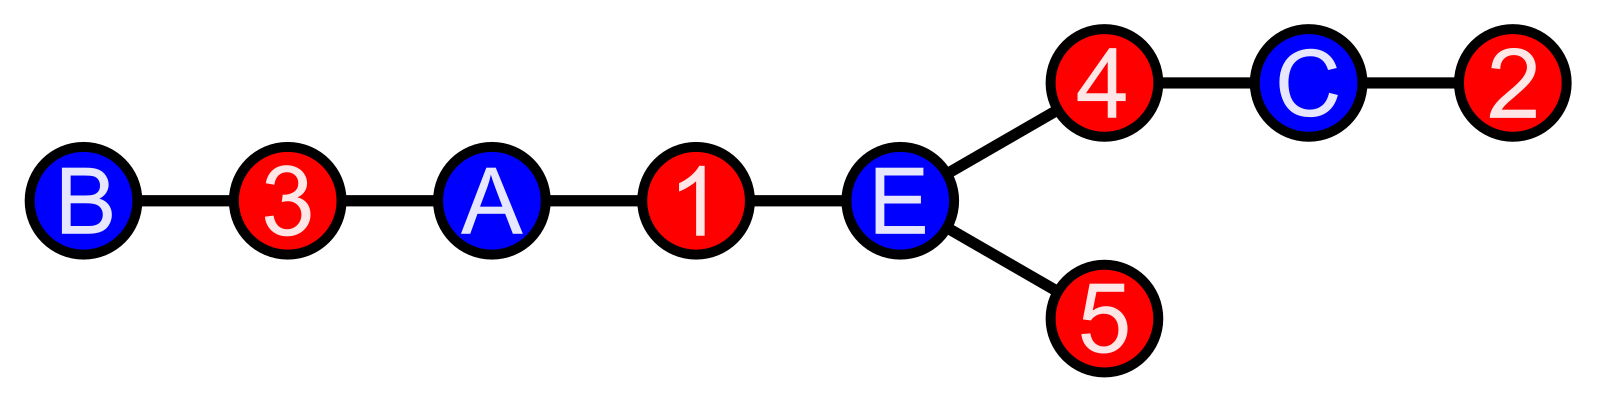
\includegraphics[scale=0.12]{bg2.png}
\end{center}
\caption{Examples of bipartife graphs with $U$ and $V$ marked in red and blue \cite{bg}}
\end{figure}

\end{CountingDefinition}

\begin{CountingDefinition}[Problem: BipartiteMatching]{def:validLabelPlacement}
Given: Bipartite graph $G=(U,V,E)$.

\ \\
Is there a perfect matching $M \subseteq E$ such that for any two edges $(u,v)$ and $(u', v')$ in $M$ $u \neq u'$ and $v \neq v'$.

\ \\
I other words: A matching in a Bipartite Graph is a set of the edges chosen in such a way that no two edges share an endpoint. The matching $M$ is called perfect if for every node in $V$ there is some edge in $M$. 
\cite{bm, book, bgm}
\end{CountingDefinition}

\begin{itemize}
\item construct bipartite graph with $n$ nodes as $n \times n$ matrix $A$
\item the element $A_{i,j}$ is a variable $x_{i,j}$ if $(i,j) \in E$
\item the element $A_{i,j}$ is 0 if $(i,j) \notin E$
\end{itemize}

\textbf{Example: }

\begin{minipage}{0.50\textwidth}

\begin{center}
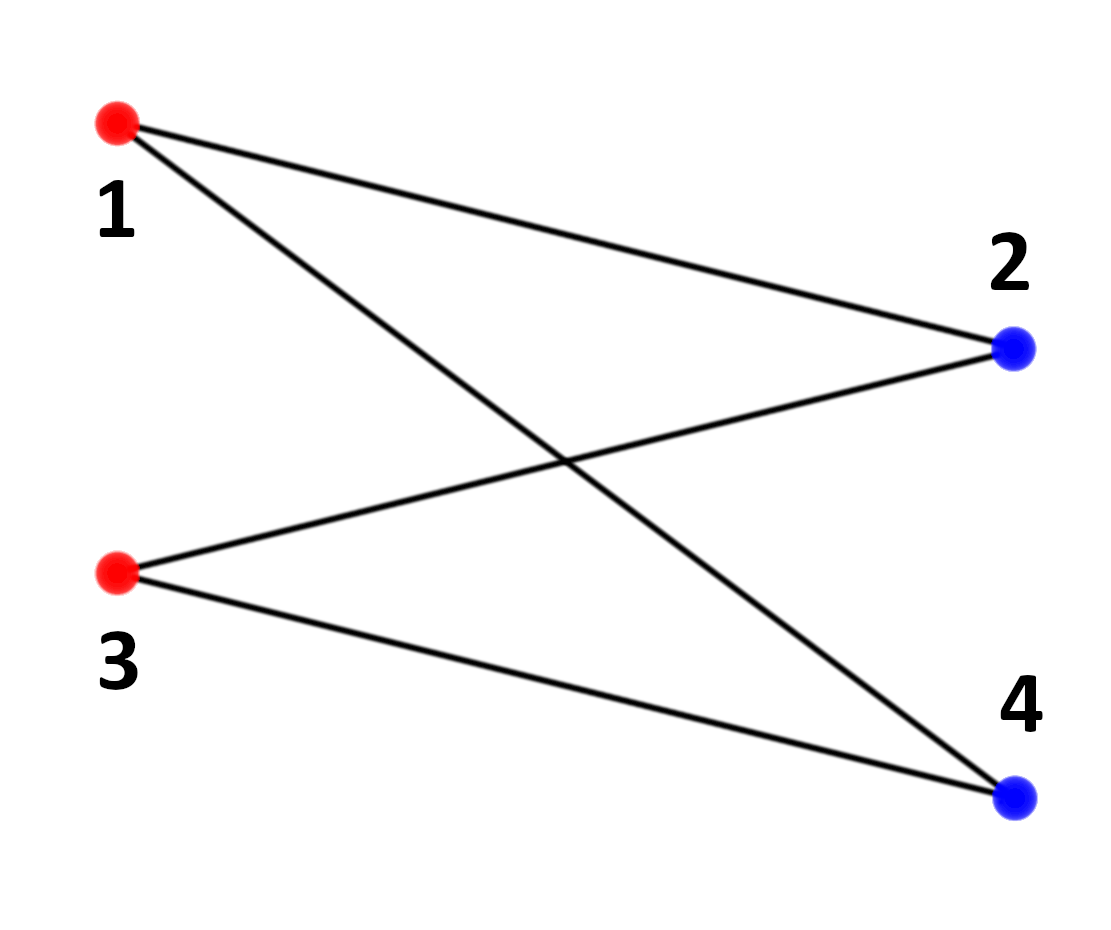
\includegraphics[scale=0.28]{v1.png}
\end{center}

\end{minipage}
\begin{minipage}{0.50\textwidth}


$ A = \begin{pmatrix}
0 & x_{1,2} & 0 & x_{1,4} \\
x_{2,1} & 0 & x_{2,3} & 0 \\
0 & x_{3,2} & 0 & x_{3,4} \\
x_{4,1} & 0 & x_{4,3} & 0
\end{pmatrix}$

\end{minipage}

\color{violet} Questions: \ \\
Is EVERY node cotained in the subset $M$ when it is a perfect matching? Does a perfect matching then only exist with an even number of vertices and $|U| = |V|$? \ \\
\color{black}
















%--------------------------------------------------------------------------------------------------------------




\subsection*{Determinant calculation}

\textbf{Leibniz-formula:}
\ \\ \ \\
\begin{minipage}{0.1\textwidth}

\ 


\end{minipage}\begin{minipage}{0.3\textwidth}
\ \\
$ A = \begin{pmatrix}
a & b & c  \\
d & e & f \\
g & h & i
\end{pmatrix}$

\end{minipage}
\begin{minipage}{0.5\textwidth}

$|A| = a \cdot e \cdot i +  b \cdot f \cdot g + c \cdot d \cdot h - g \cdot e \cdot c - h \cdot f \cdot a - i \cdot d \cdot b$


\end{minipage}

\ \\ \ \\
\begin{minipage}{0.1\textwidth}

\ 


\end{minipage}\begin{minipage}{0.3\textwidth}
\ \\
$ B = \begin{pmatrix}
1 & 2 & 3  \\
4 & 5 & 6 \\
7 & 8 & 9
\end{pmatrix}$

\end{minipage}
\begin{minipage}{0.5\textwidth}

$|B| = 1 \cdot 5 \cdot 9 +  2 \cdot 6 \cdot 7 + 3 \cdot 4 \cdot 8 - 7 \cdot 5 \cdot 3 - 8 \cdot 6 \cdot 1 - 9 \cdot 4 \cdot 2 = 0$


\end{minipage}

\begin{align*}
\\
|A| = \sum_{\pi} \sigma(\pi) \prod^{n}_{i=1} A_{i, \pi(i)}
\end{align*}
\begin{itemize}
\item $\sigma(\pi)$ decides if $+$ or $-$
\item leads to $n!$ summands
\item Example: $n= 3$ \\
$3! = 6$ summands \\
$6$ permutations for $\pi$ 
\begin{itemize}
\item[$+1$: ] $( \ 1 \ 2 \ 3 \ ) \ \ ( \ 2 \ 3 \ 1 \ ) \ \  ( \ 3 \ 1 \ 2 \ ) $
\item[$-1$: ] $( \ 3 \ 2 \ 1 \ ) \ \ ( \ 2 \ 1 \ 3 \ ) \ \  ( \ 1 \ 3 \ 2 \ ) $
\item[$\rightarrow$] $|A| = A_{1,1} \cdot A_{2,2} \cdot A_{3,3} + A_{2,1} \cdot A_{3,2} \cdot A_{1,3} + ...$
\end{itemize}
\end{itemize}



\textbf{Gaussian elimination:}
\begin{itemize}
\item Gauß algorithm for solving LSE (linear systems of equations)
\item allowed operations:
\begin{itemize}
\item addition of rwos
\item subtraction of rows
\item multiply row with integer $x$
\item divide row by integer $x$
\item switch to rows
\end{itemize}
\item wanted: upper triangular form (all entries below the diagonal 0)
\item determinant is the product of the diagonal entries
\item Example:
\begin{figure}[H]
\begin{center}
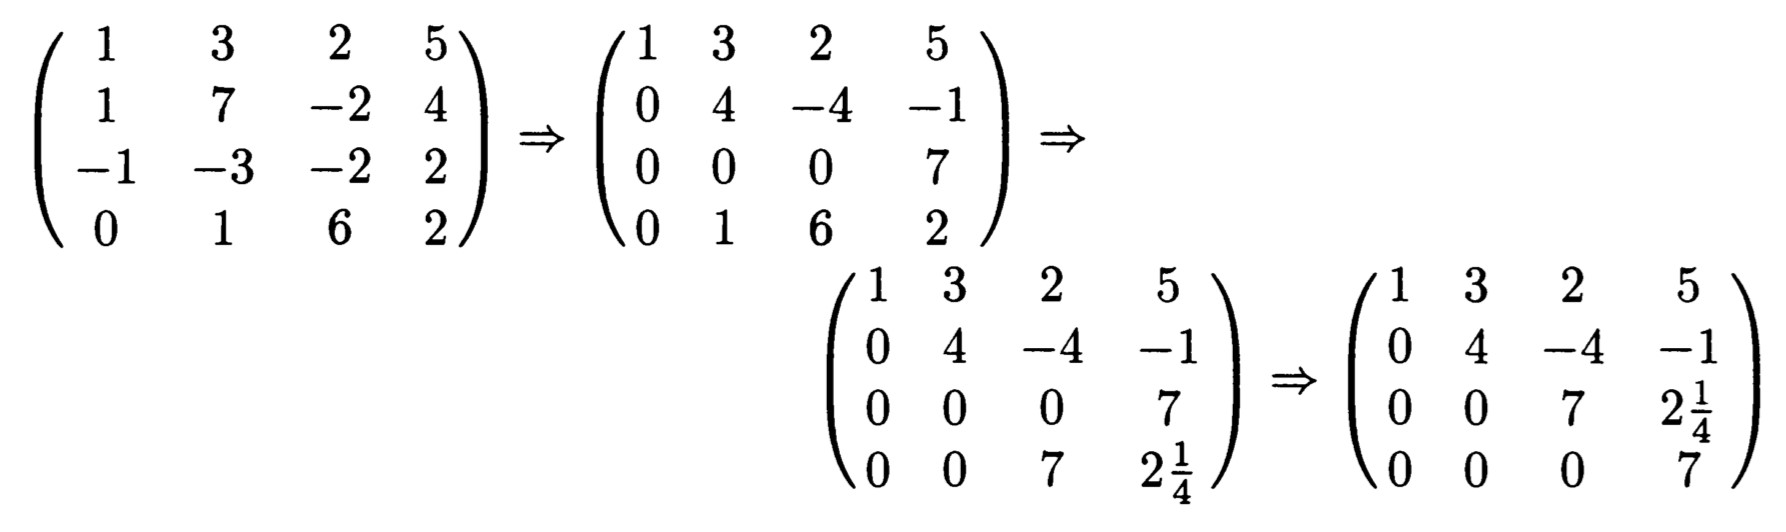
\includegraphics[scale=0.4]{gauss.jpg}
\end{center}
\caption{Examples gaussian elimination \cite{book}}
\end{figure}
$|A| = 1 \cdot 4 \cdot 7 \cdot 7 = 196$
\end{itemize}



















%-----------------------------------------------------------------------------------------------------------------------------








\subsection*{Symbolic Determinants}

Symbolic matrix: 
\begin{itemize}
\item matrix with variables instead of numerical entries
\item Example:
\begin{figure}[H]
\begin{center}
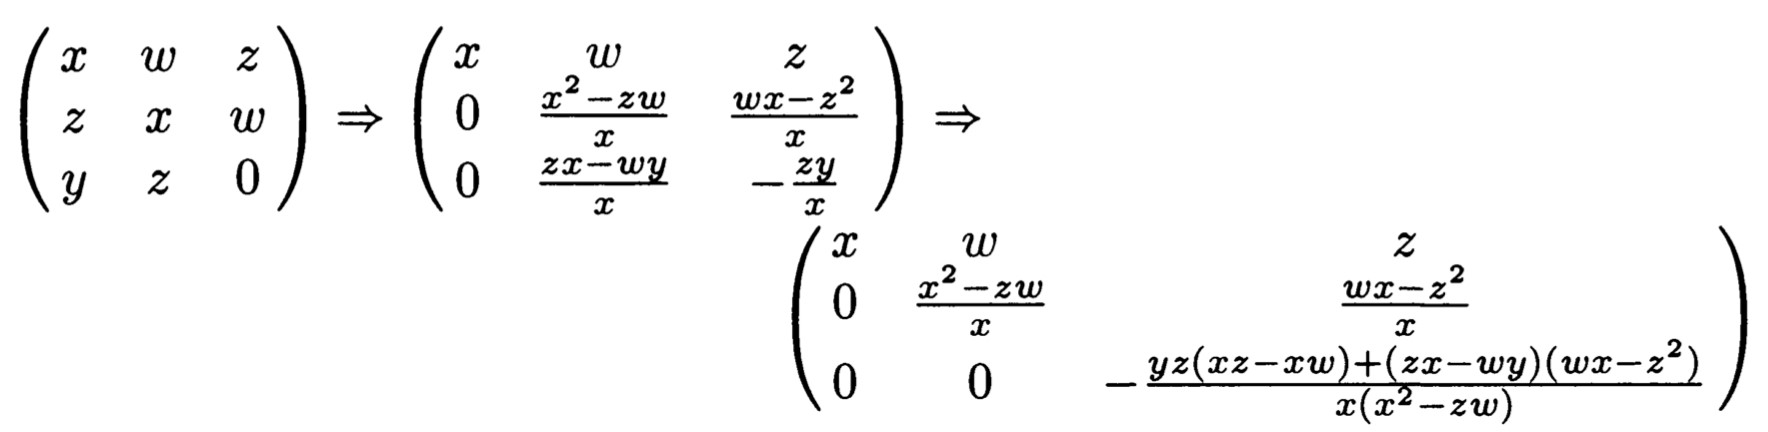
\includegraphics[scale=0.5]{gauss2.jpg}
\end{center}
\caption{Examples gaussian elimination with symbolic matrix \cite{book}}
\end{figure}
\item subdeterminants have exponentially many terms
\item wanted result: know if determinant is 0
\end{itemize}


















%-----------------------------------------------------------------------------------------------------------------------------






\subsection*{Monte Carlo algorithm}

Check if determinant of symbolic matrix is 0:
\begin{itemize}
\item use arbitrary integers for the variables \\
$\rightarrow$ numerical matrix
\item calculate determinant of numerical matrix:
\begin{itemize}
\item if not 0: \\
determinant of symbolic matrix is not 0
\item if 0: \\
determinant of symbolic matrix is probably 0
\begin{itemize}
\item numbers could be chosen such that the numrical determinant is 0 even though the symbolic one is not 0
\end{itemize}
\end{itemize}
\end{itemize}


\begin{CountingDefinition}[Monte Carlo algorithm]{def:validLabelPlacement}
Randomized algorithm for deciding if a graph $G$ has a perfect matching with calculating the determinant of the corresponding matrix $A$ to $G$.

\begin{itemize}
\item choose $m$ random integers $i_1,...,i_m$ between $0$ and $2m$
\item compute the determinant $|A|(i_1,...,i_m)$ with the Gaussian elimnation
\item if $|A|(i_1,...,i_m) \neq 0$ reply \textit{$G$ has a perfect matching}
\item if $|A|(i_1,...,i_m) = 0$ reply \textit{$G$ has probably no perfect matching}
\end{itemize}
\end{CountingDefinition}

\begin{itemize}
\item if perfect matching found: decision is reliable and final
\item if perfect matching not found: possibility of false negative
\end{itemize}

\begin{CountingDefinition}[Monte Carlo algorithm]{def:validLabelPlacement}
(Algorithm above) decides whether a symbolic matrix is \textbf{not} indentically to zero.
\end{CountingDefinition}

\textbf{Reducing chance of false negatives:}
\begin{itemize}
\item perform many independent experiments
\item chose each time random integers (independently)
\item repeat $k$ times the evaluation of the determinant of the symbolic matrix
\begin{itemize}
\item answer always zero: \\
chance that $G$ hs no perfect matching is higher ($1-(\frac{1}{2})^k$)
\item answer different from zero once: \\
perfect matching exists
\end{itemize}
\end{itemize}


\textbf{Monte Carlo algorithm:}
\begin{itemize}
\item Monte Carlo algorithm has no false positives
\item probability of false negatives is bounded
\item time needed always polynomieal
\end{itemize}




















%-----------------------------------------------------------------------------------------------------------------------------






\subsection*{Randomized complexity classes}


\begin{CountingDefinition}[Monte Carlo Turing Machine]{def:validLabelPlacement}
A polynomial Monte Carlo Turing Machine $M$ that decides a language $L$ is a nondeterministic Turing Machine with exactly two choices in each step and the following conditions:

\begin{itemize}
\item if $x \in L$ then at least half of the computations on $x$ halt with \textit{yes}
\item if $x \notin L$ then all computations halt with \textit{no}
\end{itemize}
\end{CountingDefinition}

\begin{itemize}
\item randomized algorithms can be modeled with an ordinary non-deterministic Turing Machine with different interpretation of the meaning of accepting the input
\item no false positive answers+
\item probability of false negatives is at most $\frac{1}{2}$
\end{itemize}

\begin{CountingDefinition}[RP]{def:validLabelPlacement}
Complexity class of all languages that are decided with polynomial Monte Carlo Turing Machines is denoted as RP.
\end{CountingDefinition}

\begin{itemize}
\item RP lies between P and NP (P $\subseteq$ RP $\subseteq$ NP)
\end{itemize}





\ \\

\color{red} TODO \\
More detail on definition of Monte Carlo Turing Machine. \\
Probability explanation \\
More details on RP \\
\color{black}
\color{violet} Questions: \\
More a to do than a question: More details on definition of Monte Carlo Turing Machine.
\color{black}





















%-----------------------------------------------------------------------------------------------------------------------------






\subsection*{ZPP}

\begin{CountingDefinition}[LasVegas algorithm]{def:validLabelPlacement}

The LasVegas algorithm as a Monte Carlo algorithm and its complement (one has no false positives and one has no false negatives). It runs $k$ independent experiments on both and the right answer will come up. (Either a positive answer from the one with no false positives or a negative answer from the one with no false negatives.)


\end{CountingDefinition}

\begin{itemize}
\item RP: no false positive answers but false negative answers possible
\item coRP: no false negative answers but false positive answers possible
\item RP $\cap$ coRP seems interesting:

\begin{itemize}
\item problem in this class has two Monte Carlo algorithms:
\begin{itemize}
\item one has no false positives
\item one has no false negatives
\end{itemize}
\item run enough experiments on both: right answer will come up \\
(either a positive answer from the one with no false positives or a negative answer from the one with no false negatives)
\item correct answer will be known for sure
\item execute both algorithms independent $k$ times: probability that the correct answer is not obtained is $\frac{1}{2^k}$
\item[$\rightarrow$] called LasVegas algorithm
\end{itemize}

\end{itemize}



\begin{CountingDefinition}[ZPP]{def:validLabelPlacement}
RP $\cap$ coRP 

\ \\
Complexity class of all languages that are decided with LasVegas algorithms is denoted as RP.
\end{CountingDefinition}






















%-----------------------------------------------------------------------------------------------------------------------------






\subsection*{PP}

\begin{CountingDefinition}[Problem: MAJSAT]{def:validLabelPlacement}
Given: Boolean expression $\varphi$

\ \\
Is it true that the majority of the $2^n$ truth assignments to its variables satisfy it?
\end{CountingDefinition}

\begin{itemize}
\item \textsc{MajSat} is probably not in NP
\item \textsc{MajSat} is probably not in RP
\item \textsc{MajSat} is in PP
\end{itemize}


\begin{CountingDefinition}[PP]{def:validLabelPlacement}
The class PP contains all languages $L$, such that there is a nondeterminsic polynomial Turing Machine $M$ such that for all inputs $x$: 
\begin{itemize}
\item[\ ] $x \in L$ only if more than half of the computations end up accepting (\textit{yes}).
\end{itemize}
$M$ decides $L$ by majority.
\end{CountingDefinition}

\begin{itemize}
\item P is a syntactic class (not a semantic class)
\end{itemize}

\ \\

\color{red} TODO \\
example of majsat? \\
difference between syntactic and semantic classes \\
\color{black}
\color{violet} Questions: \\
\color{black}





















%-----------------------------------------------------------------------------------------------------------------------------






\subsection*{NP $\subseteq$ PP}


\begin{itemize}
\item
\end{itemize}

\ \\

\color{red} TODO \\
\color{black}
\color{violet} Questions: \\
\color{black}
















%-----------------------------------------------------------------------------------------------------------------------------






\subsection*{BPP}

\begin{CountingDefinition}[BPP]{def:validLabelPlacement}
Answers (\textit{yes} and \textit{no}) are correct with probability $\frac{3}{4}$.
\end{CountingDefinition}

\begin{itemize}
\item
\end{itemize}

\ \\

\color{red} TODO \\
\color{black}
\color{violet} Questions: \\
\color{black}




















%-----------------------------------------------------------------------------------------------------------------------------





\subsection*{Randomized complexity classes}

\begin{figure}[H]
\begin{center}
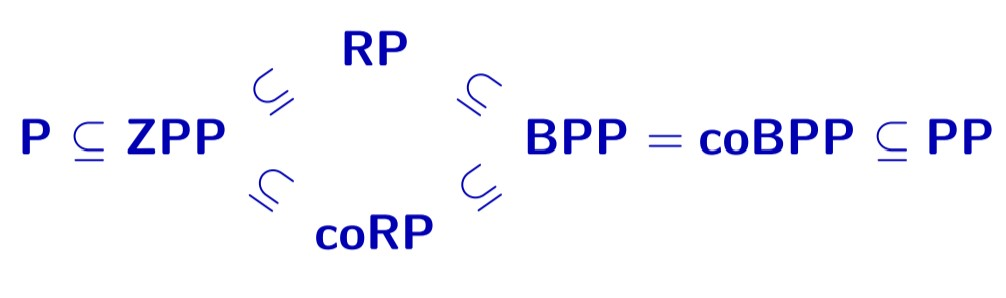
\includegraphics[scale=0.5]{cc1.jpg}
\end{center}
\caption{Relations between classes from the lecture slides \cite{CC}}
\end{figure}

\begin{figure}[H]
\begin{center}

\includegraphics[scale=0.5]{cc2.jpg}
\end{center}
\caption{Relations between classes from the lecture slides \cite{CC}}
\end{figure}

\ \\

\color{red} TODO \\
\color{black}
\color{violet} Questions: \\
\color{black}




\begin{itemize}
\item some slides about stuff that is not in the book
\item Satz von Rice
\end{itemize}


\color{red} TODO \\
some slides about stuff that is not in the book \\
Satz von Rice \\
\color{black}
\color{violet} Questions: \\
\color{black}



\newpage

\printbibliography




\end{document}